\documentclass[a4paper, 10pt, ]{article}

\usepackage[slovak]{babel}

% ------------------------------

\usepackage[utf8]{inputenc}
\usepackage[T1]{fontenc}

\usepackage[left=4cm,
            right=4cm,
            top=2.1cm,
            bottom=2.6cm,
            footskip=7.5mm,
            twoside,
            marginparwidth=3.0cm,
            %showframe,
            ]{geometry}

\usepackage{graphicx}
\usepackage[dvipsnames]{xcolor}
% https://en.wikibooks.org/wiki/LaTeX/Colors

% ------------------------------

\usepackage{lmodern}

\usepackage[tt={oldstyle=false,proportional=true,monowidth}]{cfr-lm}
% https://mirror.szerverem.hu/ctan/fonts/cfr-lm/doc/cfr-lm.pdf

% ------------------------------

\usepackage{amsmath}
\usepackage{amssymb}
\usepackage{amsthm}

\usepackage{booktabs}
\usepackage{multirow}
\usepackage{array}
\usepackage{dcolumn}

\usepackage{natbib}

% ------------------------------

\hyphenpenalty=6000
\tolerance=1000

\def\naT{\mathsf{T}}

% ------------------------------

\makeatletter

    \def\@seccntformat#1{\protect\makebox[0pt][r]{\csname the#1\endcsname\hspace{4mm}}}

    \def\cleardoublepage{\clearpage\if@twoside \ifodd\c@page\else
    \hbox{}
    \vspace*{\fill}
    \begin{center}
    \phantom{}
    \end{center}
    \vspace{\fill}
    \thispagestyle{empty}
    \newpage
    \if@twocolumn\hbox{}\newpage\fi\fi\fi}

    \newcommand\figcaption{\def\@captype{figure}\caption}
    \newcommand\tabcaption{\def\@captype{table}\caption}

\makeatother

% ------------------------------

\usepackage{fancyhdr}
\fancypagestyle{plain}{%
\fancyhf{} % clear all header and footer fields
% \fancyfoot[C]{\sffamily {\bfseries \thepage}\ | {\scriptsize\oznacenieCasti}}
\fancyfoot[C]{\sffamily {\bfseries \thepage}{\color{Gray}\scriptsize$\,$z$\,$\pageref{LastPage}}\ | 
\includegraphics[height=5pt]{../../COMMONFILES/KUT_logo_v0.1.pdf}{\scriptsize\KUTporadoveCislo}}
\renewcommand{\headrulewidth}{0pt}
\renewcommand{\footrulewidth}{0pt}}
\pagestyle{plain}

% ------------------------------

\usepackage{titlesec}
\titleformat{\paragraph}[hang]{\sffamily  \bfseries}{}{0pt}{}
\titlespacing*{\paragraph}{0mm}{3mm}{1mm}
\titlespacing*{\subparagraph}{0mm}{3mm}{1mm}

\titleformat*{\section}{\sffamily\Large\bfseries}
\titleformat*{\subsection}{\sffamily\large\bfseries}
\titleformat*{\subsubsection}{\sffamily\normalsize\bfseries}


% ------------------------------

\PassOptionsToPackage{hyphens}{url}
\usepackage[pdfauthor={},
            pdftitle={},
            pdfsubject={},
            pdfkeywords={},
            % hidelinks,
            colorlinks=false,
            breaklinks,
            ]{hyperref}


% ------------------------------

\graphicspath{%
{../fig_standalone/}%
{../../PY/fig/}%
{../../ML/fig/}%
{./fig/}%
}

% ------------------------------

\usepackage{enumitem}

\usepackage{lettrine}

% ------------------------------

\usepackage{lastpage}

\usepackage{microtype}

% ------------------------------

\usepackage{algorithm}
\usepackage[noend]{algpseudocode}
\makeatletter
\renewcommand{\ALG@name}{Algoritmus}
\makeatother
\usepackage{amsmath}
\usepackage{bbold}
\usepackage{calc}
\usepackage{dsfont}
\usepackage{mathtools}
\usepackage{tabto}


\newcommand{\mr}[1]{\mathrm{#1}}
\newcommand{\bs}[1]{\boldsymbol{#1}}
\newcommand{\bm}[1]{\mathbf{#1}}

\newcommand{\diff}[2]{\frac{\Delta #1}{\Delta #2}}
\newcommand{\der}[2]{\frac{d #1}{d #2}}
\newcommand{\parder}[2]{\frac{\partial #1}{\partial #2}}

\newcommand{\argmax}[0]{\mr{argmax}}
\newcommand{\diag}[0]{\mr{diag}}
\newcommand{\rank}[0]{\mr{rank}}
\newcommand{\trace}[0]{\mr{tr}}

\renewcommand{\Re}{\mr{Re}}
\renewcommand{\Im}{\mr{Im}}


\theoremstyle{definition}
\newtheorem{definition}{Definícia}[section]
\newtheorem{theorem}{Veta}[section]
\newtheorem{lemma}[theorem]{Lemma}
\newtheorem{example}{Príklad}[section]
\renewcommand*{\proofname}{Dôkaz}

% ------------------------------

\usepackage{siunitx}

% -----------------------------------------------------------------------------

\def\oznacenieCelku{Kolekcia učebných textov}

% -----------------------------------------------------------------------------


\def\KUTporadoveCislo{devAS3}

\def\oznacenieVerzie{v1.0}
% \def\oznacenieVerzie{\phantom{v1.0}}

\def\mesiacRok{august 2025}

\def\authorslabel{RJ}



\newcommand{\figref}[1]{\hyperref[#1]{obr.~\ref*{#1}}}

% Tables: "tab. 1"
\newcommand{\tabref}[1]{\hyperref[#1]{tab.~\ref*{#1}}}

% Equations: "rov. (1)"
\newcommand{\eqrefsk}[1]{\hyperref[#1]{rov.~(\ref*{#1})}}


% -----------------------------------------------------------------------------

\begin{document}

% -----------------------------------------------------------------------------
% Uvodny nadpis

\noindent
\parbox[t][18mm][c]{0.3\textwidth}{%
    \raisebox{-0.9\height}{%
        \phantom{.}
\includegraphics[height=18mm]{./COMMONFILES/URKFEIlogo.pdf}%
    }%
}%
\parbox[t][18mm][c]{0.7\textwidth}{%
    \raggedleft

    \sffamily
    \fontsize{16pt}{18pt}
    \fontseries{sbc}
    \selectfont

    \noindent
    \textcolor[rgb]{0.75, 0.75, 0.75}{\textls[25]{\oznacenieCelku}}
}%

\noindent
\parbox[t][16mm][b]{0.5\textwidth}{%
    \raggedright

    \color{Gray}
    \sffamily

    \fontsize{12pt}{12pt}
    \selectfont
    \mesiacRok

    \fontsize{6pt}{10pt}
    \selectfont
    \href{https://github.com/OkoliePracovnehoBodu/KUT}{github.com/OkoliePracovnehoBodu/KUT}

    \fontsize{8pt}{10pt}
    \selectfont
    \authorslabel




}%
\parbox[t][16mm][b]{0.5\textwidth}{%
    \raggedleft

    \sffamily

    \fontsize{6pt}{6pt}
    \selectfont

    \textcolor[rgb]{0.68, 0.68, 0.68}{\oznacenieVerzie}


    \fontsize{14pt}{14pt}
    \selectfont

    \bfseries

    
\includegraphics[height=12pt]{./COMMONFILES/KUT_logo_v0.1.pdf}%
    {%
        \textls[-50]{\KUTporadoveCislo}
    }%
}%

% -----------------------------------------------------------------------------




\vspace{6mm}

% ---------------------------------------------
\sffamily
\bfseries
\fontsize{18pt}{21pt}
\selectfont

\begin{flushleft}
    Laboratórne zariadenie AeroShield:\\ statická charakteristika
\end{flushleft}

\bigskip

% -----------------------------------------------------------------------------
\normalsize
\normalfont
% -----------------------------------------------------------------------------

\lstset{style=mystyle}










\noindent
\lettrine[lines=1, nindent=1pt, loversize=0.0]{C}{ieľom}
textu je opis a príklad merania statickej charakteristiky (prevodová charakteristika) pre AeroShield zariadenie.


\section{Postup návrhu merania statickej charakteristiky}

AS je laboratórne zariadenie predstavujúce reálny dynamický systém, ktorý sme predstavili v \href{run:../../KUTdev_AeroShield_Info/TeX/KUTdevAS0.pdf}{KUT dokumente Laboratórne zariadenie AeroShield:\\ orientačný prehľad}. V prípade, že chceme odmerať statické vlastnosti systému, musíme vedieť rozsahy vstupov a výstupov, aby sme boli schopný korektne navrhnúť experiment na zmeranie vlastností systému.
V prípade AS vieme, že vstupný signál je v rozsahu $0\% - 100\%$, musíme si zvoliť rozumnú veľkosť kroku a dĺžku trvania kroku, aby sme dostatočne zachytili vlastnosti systému. Zvoľme si teda podľa tab. \ref{tab:config}.

\begin{center}

    \vspace{-10pt}

    \tabcaption{Nastavenia merania}
    \label{tab:config}

    \lstyle

    \begin{tabular*}{\textwidth}{@{ \extracolsep{\fill}} lll}
        \toprule
        Nastavenie & Hodnota & Jednotka \\
        \midrule
        Veľkosť kroku & $1$ & \% \\
        Trvanie & $10$ & s \\
        \bottomrule
    \end{tabular*}

\end{center}

Nakoľko meriame statické vlastnosti, tak nás zaujíma iba priebeh výstupného signálu v \emph{ustálenom stave}. Teda keď systém neprejavuje žiadne dynamické vlastnosti, t.j. neprebieha žiaden nami vyžiadaný dynamický dej.

% Bolo by fajn sa pokusit nejak zadefinovat pojem ustaleny stav.
% Čo považujeme za ustálený stav podrobnejšie najdete v KUT ustálený stav.


\section{Meranie statickej charakteristiky}
Veľkosť kroku si volíme podľa potreby, v rámci merania sme vybrali veľkosť kroku $1$, nakoľko sme chceli ukázať, nelinearity systému t.j. \emph{deadzone} (suché trenie) a \emph{saturation} (saturácia/ohraničenie). Stojí nás to čas trvania merania (viď \figref{fig:ss_raw}), však v realite, by sme meranie zastavili hneď po dovršení konečnej saturácie, nakoľko chceme predísť možným poškodeniam systému alebo okoliu.

\begin{center}

    \vbox{%


        \makebox[\textwidth][c]{%
            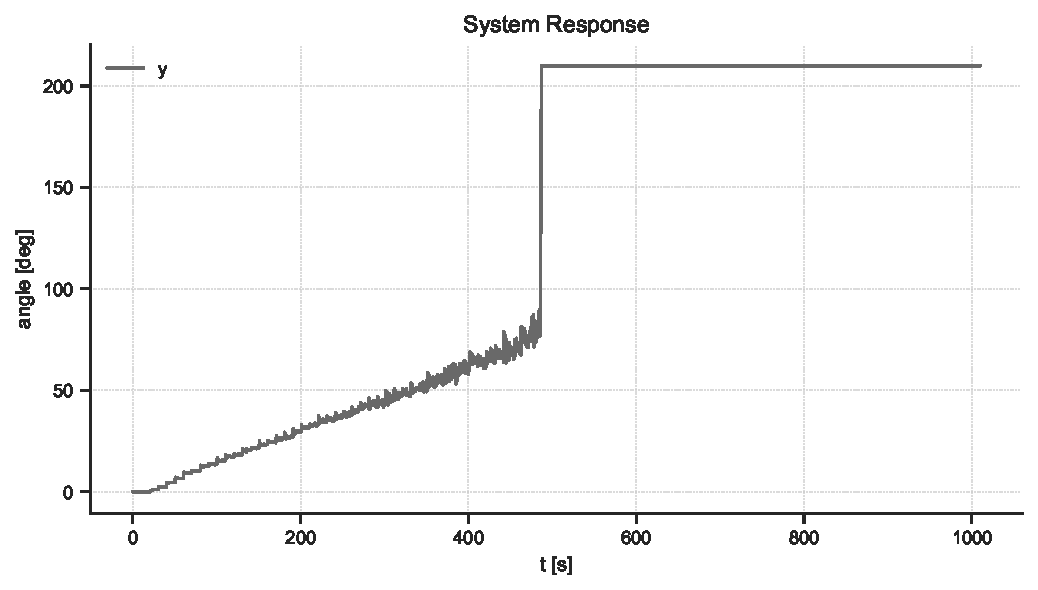
\includegraphics{measurement.pdf}
        }

        \figcaption{
            Priebeh merania statickej charakteristiky.
        }
        \label{fig:ss_raw}
    }%vbox

\end{center}

Ako si možeme všimnúť na \figref{fig:ss_raw} v okolí $t = 0$ a $t = 500$ sa prejavujú nelinearity systému, ktoré chceme v rámci identifikácie lineárneho modelu systému opomenúť, nakoľko sú \emph{nelineárne}. Možno lepšie znázorniť nelineárne časti systému, použitím iného spôsobu náhladu dát \figref{fig:ss_raw_gain}.

\begin{center}

    \vbox{%


        \makebox[\textwidth][c]{%
            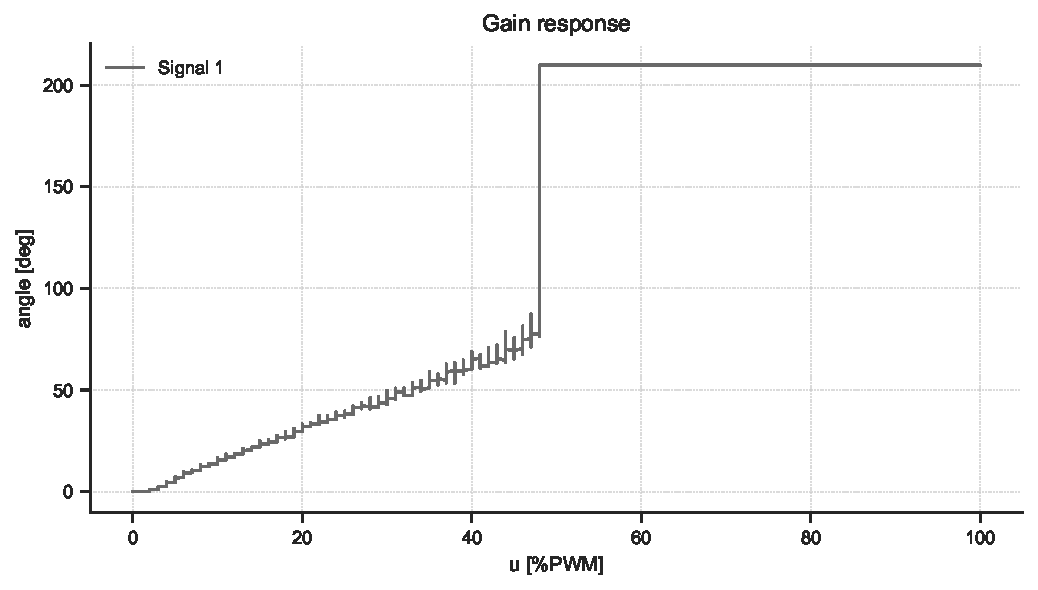
\includegraphics{gain_response.pdf}
        }

        \figcaption{
            Vstupno-výstupná charakteristika.
        }
        \label{fig:ss_raw_gain}
    }%vbox

\end{center}

\section{Spracovanie merania statickej charakteristiky}
Ako sme spomínali, chceme odstrániť nelinearnej časti, z ktorých si vieme následne vyčítať hodnoty nelinearít, ktoré vieme následne využiť pri identifikácii a konštrukcii nelineárneho modelu systému. V tejto časti však chceme dostať model statickej charakteristiky zariadenia, postup je následovný.

\begin{enumerate}

\item Získame si intervaly merania, kedy je výstupný signál systému ustálený.
\item Použijeme vhodné kritérium na vyhodnotenie ustálenej hodnoty systému pre jednotku akčného zásahu. (stredná hodnota)
\item Priradíme si vypočítanú ustálenú hodnotu systému ku veľkosti akčného zásahu.
\item Následne vykreslíme hodnoty ustálených hodnôt a akčných zásahov, čo predstavuje statickú charakteristiku systému.
\item Model vytvoríme z kvázi lineárnej časti statickej charakteristiky, z ktorej si vyberáme pracovné body.
\item Odstránime nelinearity, ktoré by spôsobovali vysoký rád modelu.
\item Nakoniec optimálne spojimé vyhodnotené body výstupnej veličiny v závislosti od akčého zásahu. (Nafitujeme polynomickú funkciu n-tého rádu na konečné dáta)

\end{enumerate}

\begin{center}

    \vbox{%


        \makebox[\textwidth][c]{%
            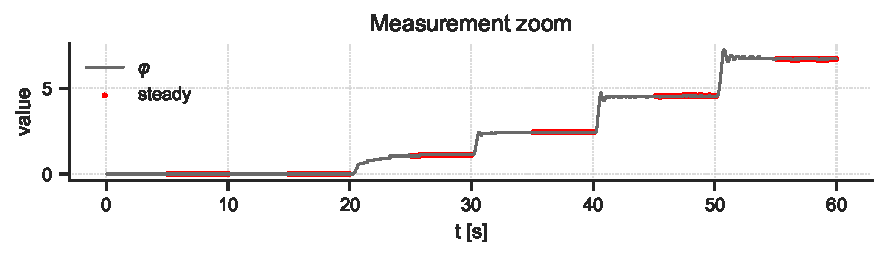
\includegraphics{measurement_zoom.pdf}
        }

        \figcaption{
            Detail nameraných dát a zobrazenie intervalov ustálených hodnôt merania.
        }
        \label{fig:ss_raw_zoom}
    }%vbox

\end{center}

Na \figref{fig:ss_raw_zoom} je detail začiatku merania, na ktorom vyznačujeme intervaly ustálených hodnôt merania, v našom prípade merania sme si zadefinovali, že ustálenie nastáva v $50\%$ dĺžky trvania skoku. V inom prípade, by sme museli buď zaviesť nové kritérium pre nájdenie kvázi ustáleného stavu alebo ručne pre každé meranie vyznačiť interval. Kritérium derivácie rovnej 0 alebo konštante nemožno v realite použiť bez rôznych ošetrení, nakoľko do meraniu vstupujú vonkajšie vplyvy, ktoré zašumia snímaný signál a teda vnášajú nepresnosť do merania a spracovania dát.

Následne sme použili jednoduchý výpočet strednej hodnoty množiny výstupných hodnôt v intervale ustálených výstupných hodnôt, čo je znázornené na \figref{fig:ss_char}, kde sme priradili stredné hodnoty ustalených hodnôt k vstupnej veličine teda akčnému zásahu.


\begin{center}

    \vbox{%


        \makebox[\textwidth][c]{%
            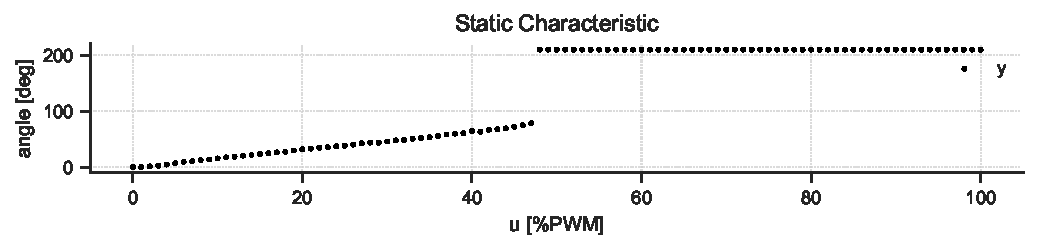
\includegraphics{ss_char_gain.pdf}
        }

        \figcaption{
            Statická (Prevodová) charakteristika zariadenia AeroShield.
        }
        \label{fig:ss_char}
    }%vbox

\end{center}


Nakoniec vytvoríme jednoduchý polynomický model statickej charaktertistiky, ktorý nám posluži pri predikcii ustáleného stavu pre naše zariadenie. Odstránime nelineárne časti - teda body, ktoré nevieme preložiť jednoduchou priamkou od počiatočne zvoleného bodu po koncovo zvolený bod, nakoľko v našom prípade by model bol vysokého rádu pri ponechaní nelinearít - viac ako 10. rád. Takto sme si zjednodušili model, vypočtovú náročnosť a zanedbali sme vonkajšie poruchy, ktoré nám skreslujú meranie a model. Vybrali sme si identifikovať model 3. rádu (viď \eqref{eq:poly_model}), nakoľko v pomere náročnosť a presnosť je postačujúci. Náš navrhovaný model vyzerá nasledovne:

\begin{equation}
    y(u) = b_3 u^3 + b_2 u^2 + b_1 u + b_0.
    \label{eq:poly_model}
\end{equation}

Po použití funkcie \emph{polyfit}, sme dostali výsledný vzťah:

\begin{equation}
    y(u) = 0.0004 u^3 + (-0.0289) u^2 + 2.1281 u + (-3.3064).
    \label{eq:poly_model_full}
\end{equation}

Následne, keď do modelu \eqref{eq:poly_model_full} dosadime hodnoty akčných zásahov, v rozmedzí intervalu, ktoré sme nemerali napr. hodnotu $u = 15.5$, dostaneme približnú hodnotu, na ktorej sa reálne zariadenie ustály, pri danej hodnote akčného zásahu. Tento model je znázornený na \figref{fig:ss_char_model} bodmi, zatiaľ čo namerané hodnotý červenými krížíkmi. Dodatočne sme vyjadrili chybovosť modelu pomocou kritéria priemeru rozdielu štvorcou (Mean Square Error \emph(MSE)).

\begin{center}

    \vbox{%


        \makebox[\textwidth][c]{%
            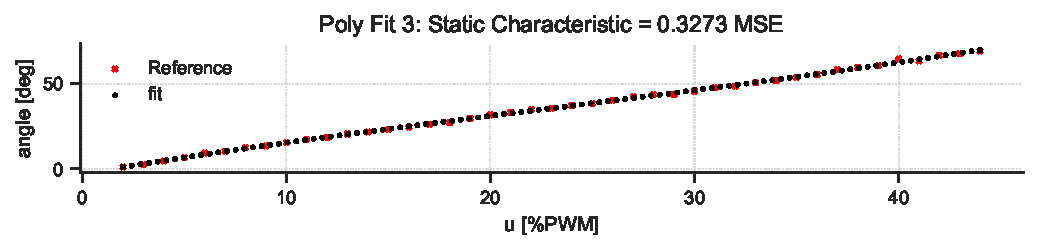
\includegraphics{ss_char_polyfit.pdf}
        }

        \figcaption{
            Identifikovaný polynomický model statickej charakteristiky 3. rádu.
        }
        \label{fig:ss_char_model}
    }%vbox

\end{center}



% -----------------------------------------------------------------------------

\end{document}

% -----------------------------------------------------------------------------